\documentclass{beamer}
\usepackage[utf8]{inputenc}
\usepackage[french]{babel}
\usepackage[T1]{fontenc}
\usepackage{amsmath}
\usepackage{amsfonts}
\usepackage{csquotes}
\usepackage{amssymb}
\usepackage{graphicx}

\usetheme{Szeged}
\usepackage{xcolor}
\definecolor{mygreen}{RGB}{46,139,87}
\setbeamercolor{structure}{fg=mygreen}
\usefonttheme{structuresmallcapsserif}

\usepackage[style=authoryear-comp, backend=biber, natbib=false]{biblatex}
\addbibresource{../latex_report/references.bib}

\setbeamertemplate{footline}[frame number]

\setbeamertemplate{bibliography item}{}
\setbeamerfont{bibliography entry author}{size=\small, series=\bfseries}
\setbeamerfont{bibliography entry title}{size=\small}
\setbeamerfont{bibliography entry journal}{size=\small, shape=\itshape}
\setbeamerfont{bibliography entry note}{size=\footnotesize}

\setlength{\bibitemsep}{0.8em}
\setlength{\bibhang}{0em}

\renewcommand*{\nameyeardelim}{\addcomma\space}

\title{ADAM pour le Deep Learning}
\author{ACHIQ Aya, CLETZ Laura, EL MAZZOUJI Wahel}

\date{\footnotesize Octobre 2025}

\titlegraphic{ 
\centering

\includegraphics[height=1.2cm]{../latex_report/images/UM.png}\hspace{0.3cm}%

\includegraphics[height=1.2cm]{../latex_report/images/SSD.png}\hspace{0.3cm}%

\includegraphics[height=1.2cm]{../latex_report/images/FdS.jpg}
}

\begin{document}

\begin{frame}

  \titlepage
  %logo 

\end{frame}

\begin{frame}{Sommaire}

  \tableofcontents

\end{frame}

\section{Enjeux et cadre statistique}

\begin{frame}{Optimisation en Deep Learning}

  \begin{itemize}
    \item But : minimiser le fonction de \textbf{perte} $\mathcal{L}(\theta)$ pour un poids $\theta$.
    \medskip
    \item Enjeux : 
    \begin{itemize}
      \item Convergence rapide ;
      \item Stabilité numérique ;
      \item Bonne généralisation.
    \end{itemize}
  \end{itemize}
  
  \begin{center}
    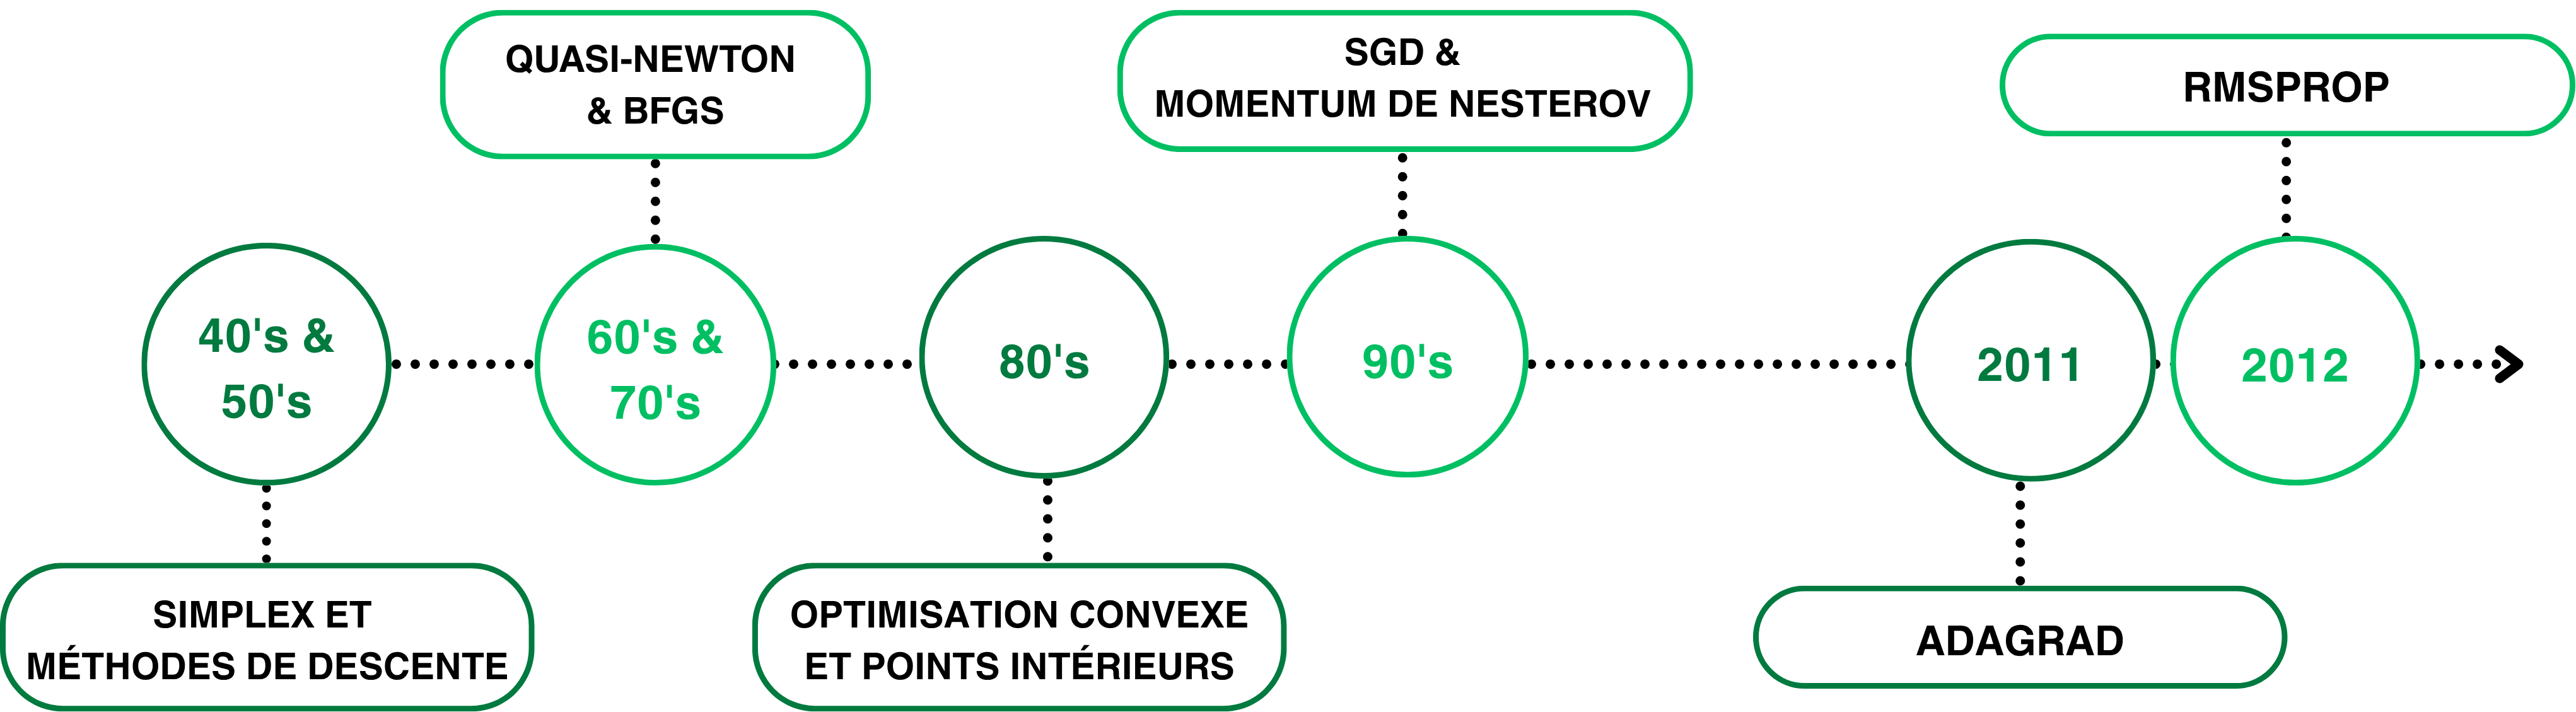
\includegraphics[width=\textwidth]{frise1.png}
  \end{center}

\end{frame}

\begin{frame}{Optimisation en Deep Learning}

  \begin{itemize}
    \item But : minimiser le fonction de \textbf{perte} $\mathcal{L}(\theta)$ pour un poids $\theta$.
    \medskip
    \item Enjeux : 
    \begin{itemize}
      \item Convergence rapide ;
      \item Stabilité numérique ;
      \item Bonne généralisation.
    \end{itemize}
  \end{itemize}
  
  \begin{center}
    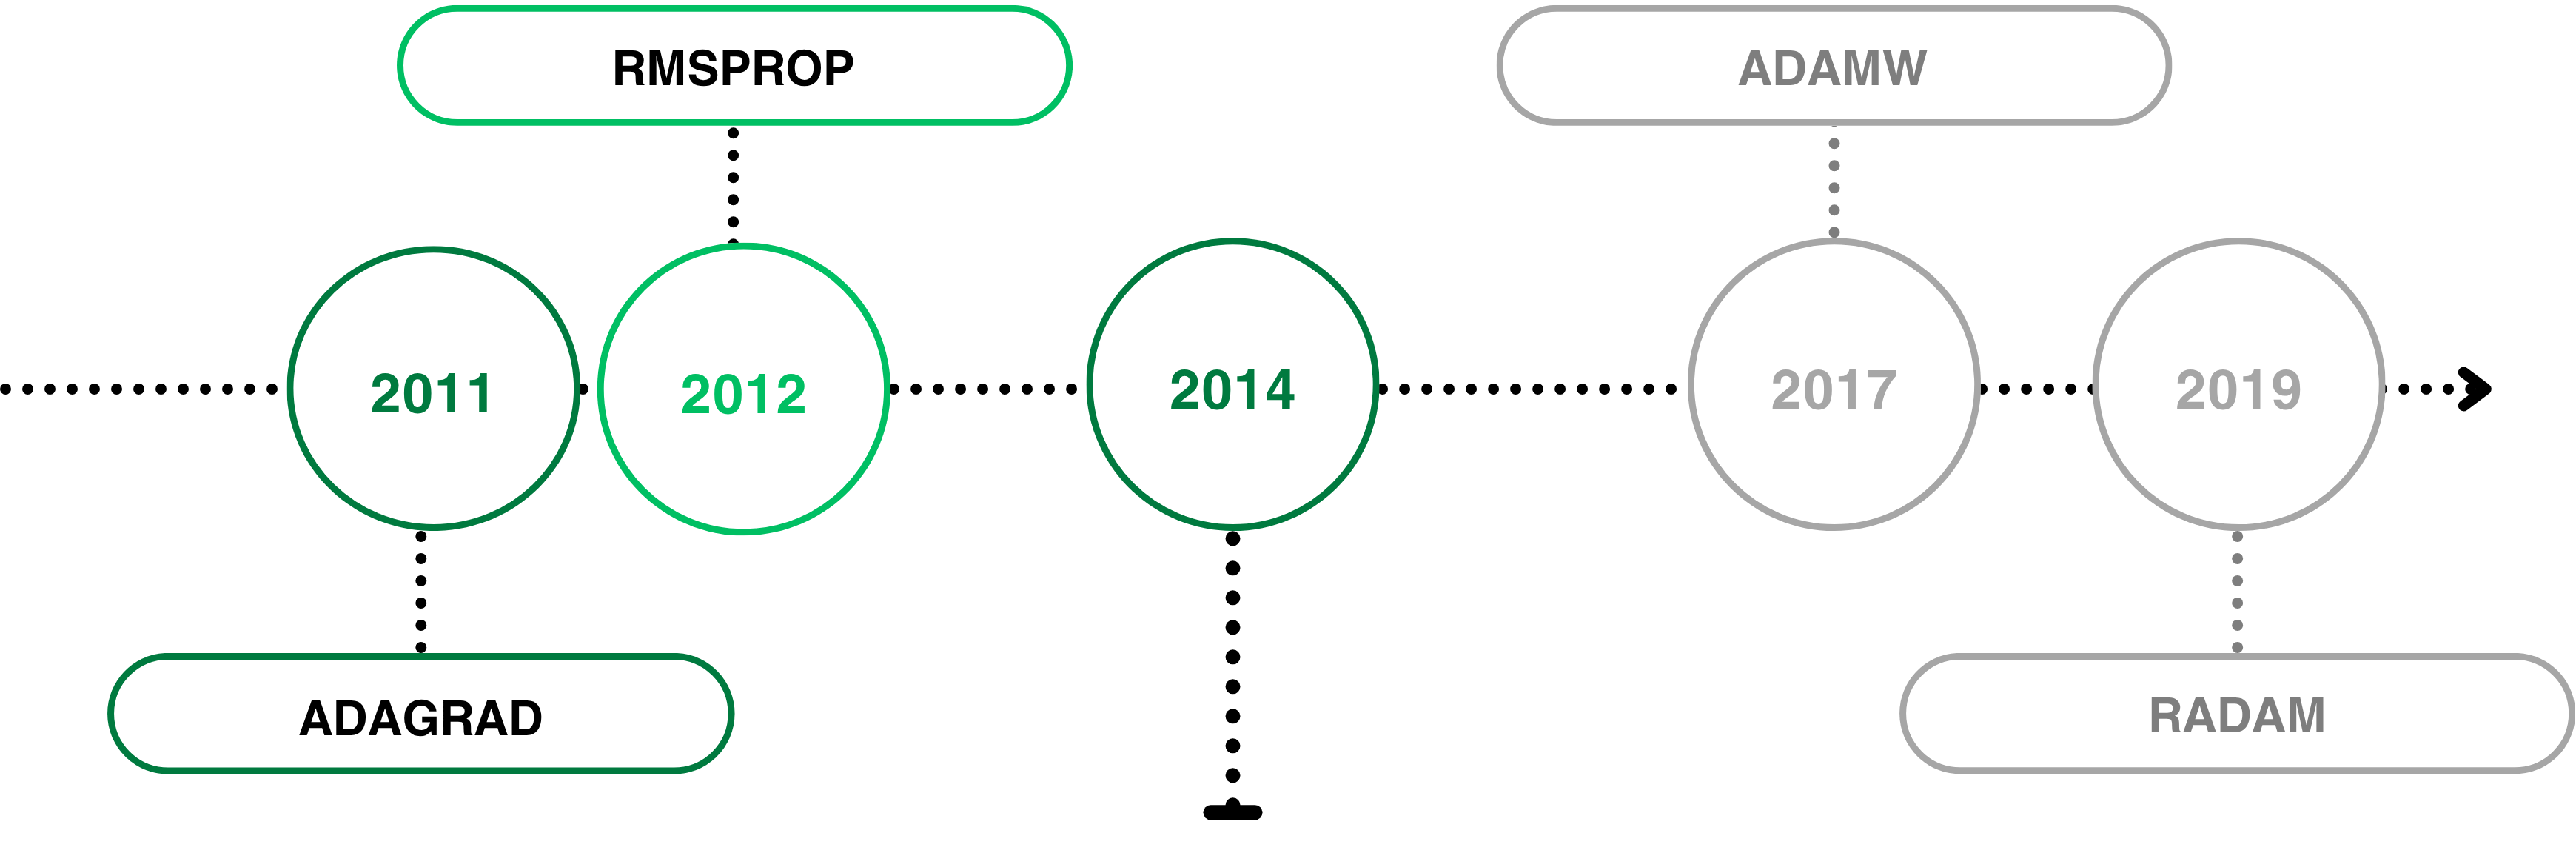
\includegraphics[width=0.8\textwidth]{frise2.png}
  \end{center}

  \begin{center}
    ADAM, \cite{kingma2014}
  \end{center}
  \begin{itemize}
    \item Est-ce l’algorithme d’optimisation idéal pour le Deep Learning ?
  \end{itemize}

\end{frame}

%-------------------------------------------------------------

\begin{frame}{Notions d'optimisation}

  \begin{itemize}
    \item Notations :
    \begin{itemize}
      \item Le gradient $g_t = \nabla_{\theta} \mathcal{L}(\theta_{t-1})$ ;
      \item Le \textbf{learning rate} $\eta$ : contrôle la taille des \textbf{pas} de mise à jour des paramètres, diffère suivant la méthode (\cite{ruder2016overview}) ;
      \item Le \textbf{momentum} $m_t$ : lissage de la trajectoire des gradients, calculé à partir de $g_{t-1}$.
    \end{itemize}
  \end{itemize}

  \begin{center}
    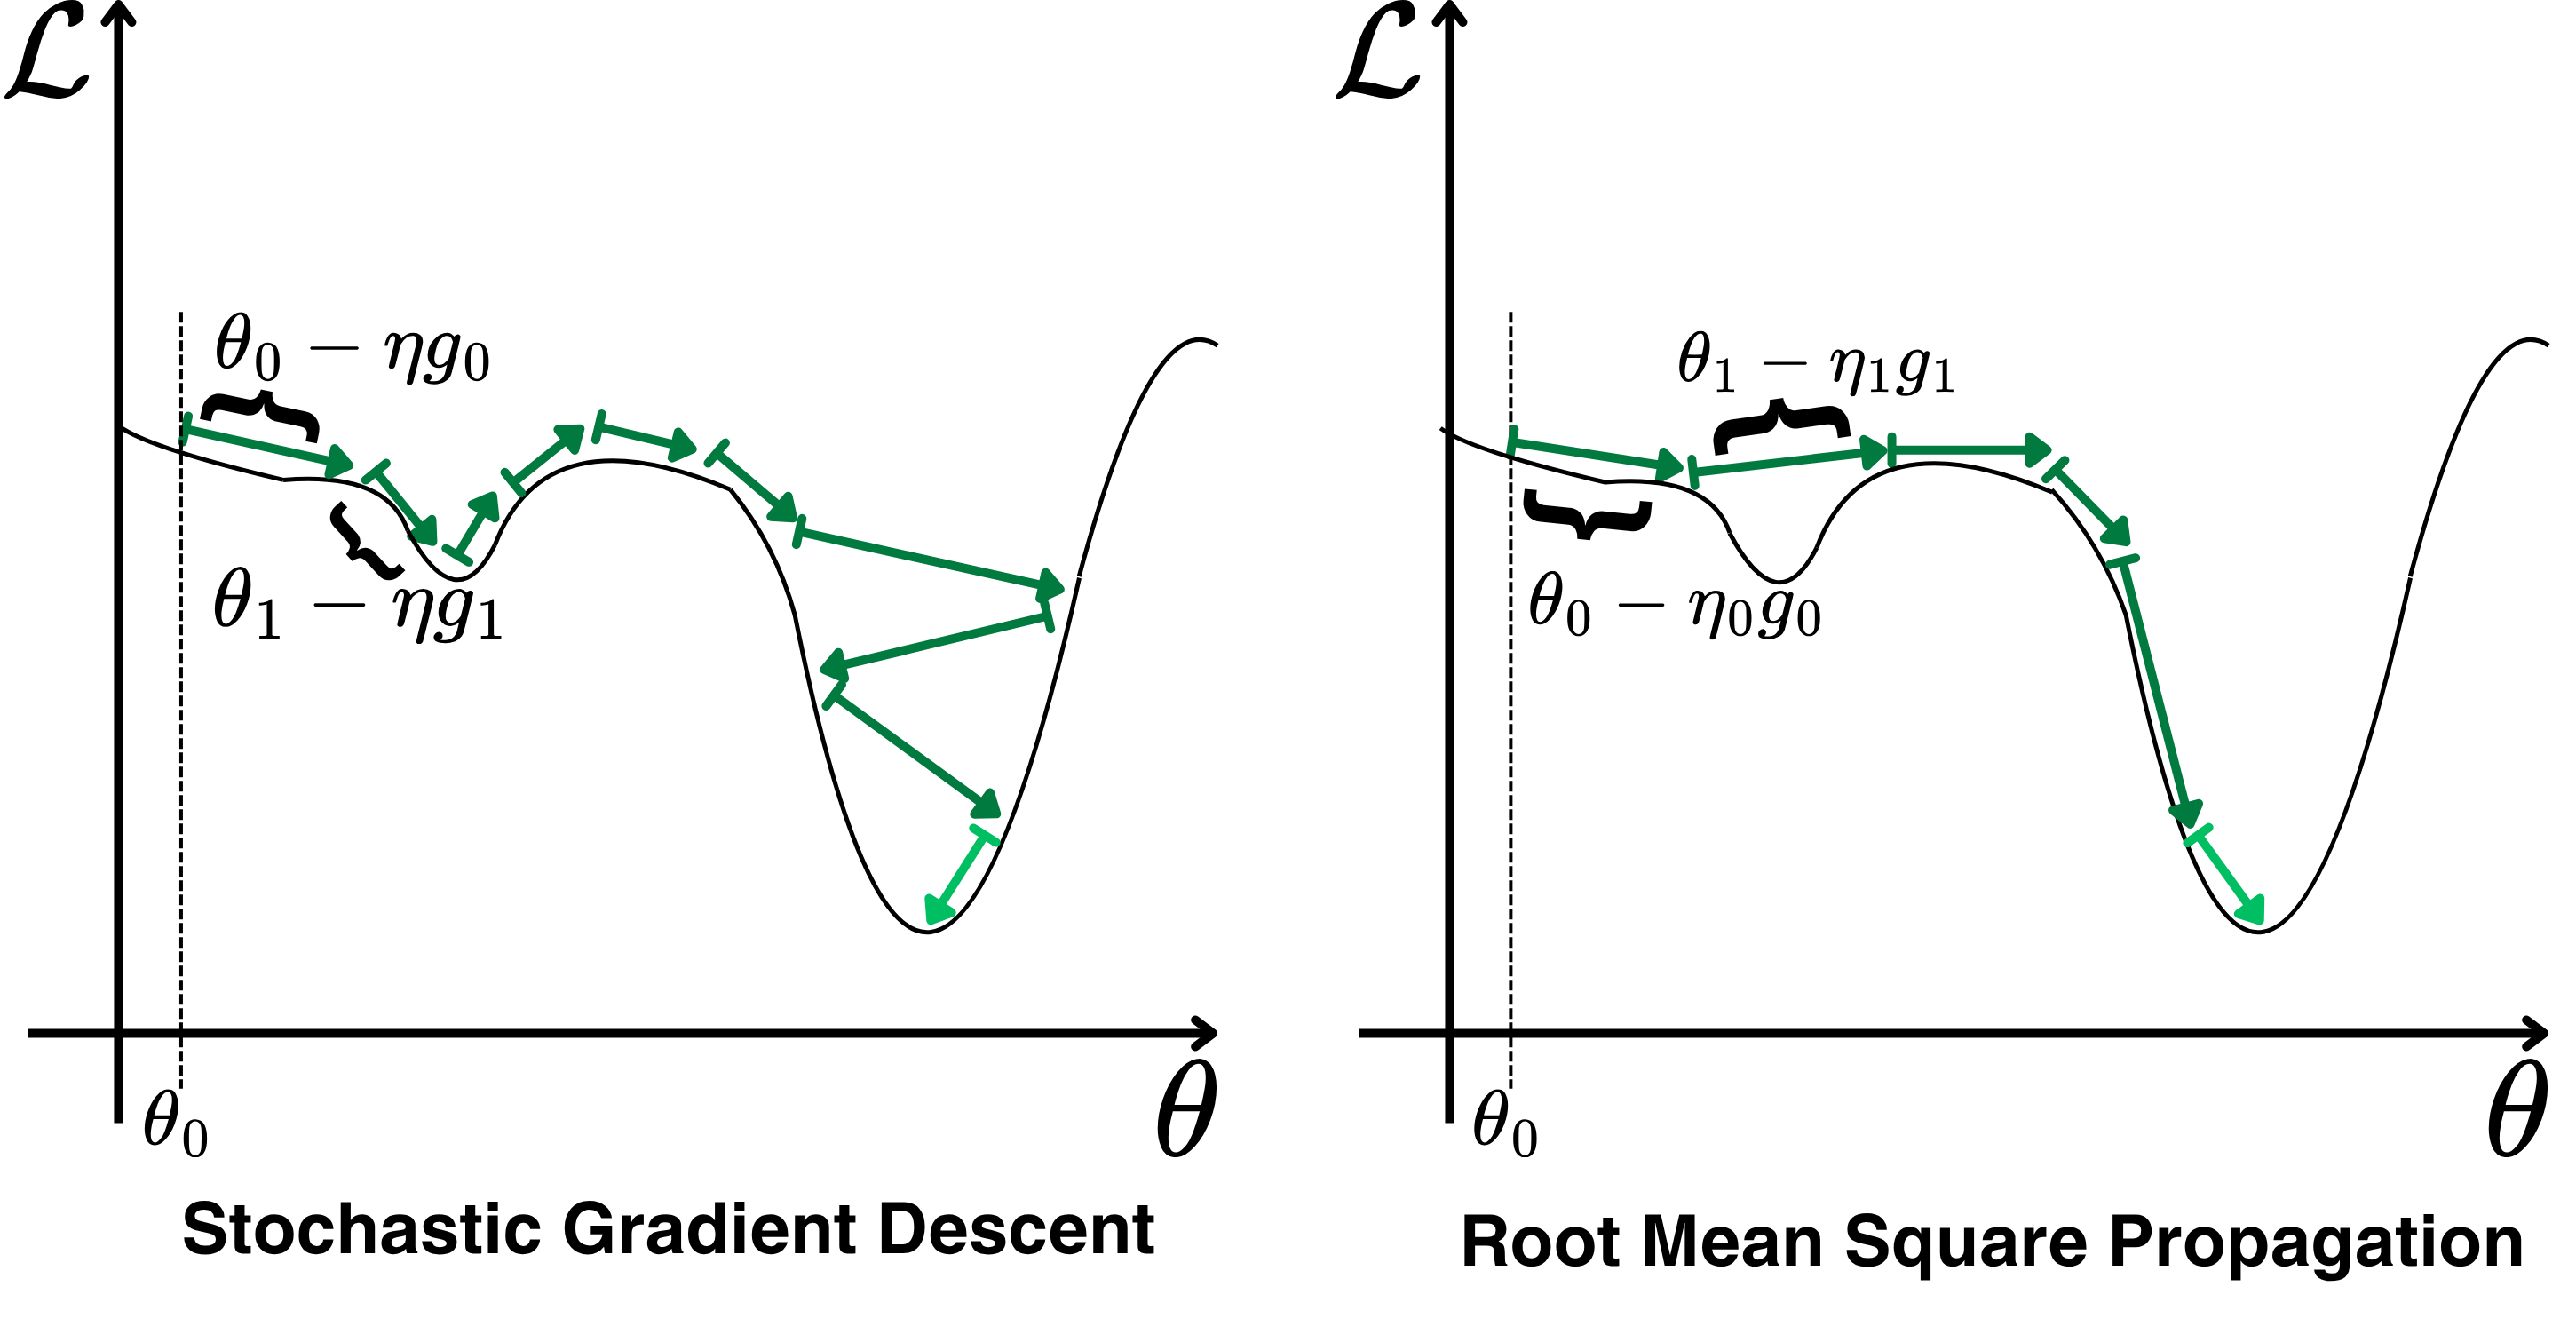
\includegraphics[width=0.8\textwidth]{SGD_RMSProp.png}
  \end{center}

\end{frame}

%-------------------------------------------------------------

\begin{frame}{Principe de l’algorithme Adam}

\begin{block}{Idée clé}
\textbf{Adam = Adaptive Moment Estimation} :
combine le \textcolor{mygreen}{momentum} et une \textcolor{mygreen}{adaptation du pas} pour chaque paramètre.
\end{block}

\bigskip

\begin{itemize}
  \item Moyennes mobiles :
    \[
      m_t = \beta_1 m_{t-1} + (1 - \beta_1) g_t, \quad
      v_t = \beta_2 v_{t-1} + (1 - \beta_2) g_t^2
    \]
  \item Mise à jour :
    \[
      \theta_t = \theta_{t-1} - \alpha \frac{\hat{m}_t}{\sqrt{\hat{v}_t} + \varepsilon}
    \]
  \item Valeurs typiques : $\alpha{=}0.001$, $\beta_1{=}0.9$, $\beta_2{=}0.999$.
\end{itemize}

\bigskip

\textbf{Propriétés :}
invariance d’échelle, stabilité, faible sensibilité aux hyperparamètres.

\end{frame}

%-------------------------------------------------------------

\section{Forces et faiblesses}

\begin{frame}{Objectifs et limites d’Adam}

\begin{columns}[T]
\column{0.48\textwidth}
\textbf{Objectifs :}
\begin{itemize}
  \item Améliorer la convergence en combinant momentum et taux d’apprentissage adaptatif ;
  \item Stabiliser l’apprentissage, même lorsque les gradients sont bruités ;
  \item Réduire la sensibilité aux hyperparamètres grâce à l’adaptation automatique des pas.
\end{itemize}

\column{0.48\textwidth}
\textbf{Limites :}
\begin{itemize}
  \item Moindre généralisation que SGD \cite{wilson2017} ;
  \item Convergence vers $\|w\|_\infty$ minimale ;
  \item Compromis entre vitesse et généralisation.
\end{itemize}
\end{columns}

\end{frame}


\begin{frame}{Expérimentation : Méthodologie}

\begin{columns}[T]

\column{0.48\textwidth}
\begin{block}{Credit Card}
\small
\begin{itemize}
  \item Taille : \textbf{10k / 100k}
  \item Features : \textbf{2} 
  \item Classes : Déséquilibrées
  \item Réseau : {[}2→8→4→1{]}
\end{itemize}
\textcolor{mygreen}{$\rightarrow$ Dataset large, simple}
\end{block}

\column{0.48\textwidth}
\begin{block}{Heart Disease}
\small
\begin{itemize}
  \item Taille : \textbf{1025}
  \item Features : \textbf{13}
  \item Classes : Équilibrées
  \item Réseau : {[}13→16→8→1{]}
\end{itemize}
\textcolor{mygreen}{$\rightarrow$ Dataset petit, complexe}
\end{block}

\end{columns}

\vspace{0.5cm}

\textbf{Optimiseurs :} Adam, SGD, Adagrad, RMSprop \\
\textbf{Learning rates :} 0.001 (Adam/RMSprop), 0.01 (SGD/Adagrad)

\end{frame}

\begin{frame}{Credit Card Fraud Detection}

\begin{columns}[T]

\column{0.48\textwidth}
\begin{center}
\textbf{n = 10~000}
\end{center}
\vspace{-0.7cm}
\begin{center}
\footnotesize
\begin{tabular}{|l|c|c|}
\hline
\textbf{Optimiseur} & \textbf{Loss} & \textbf{Erreur (\%)} \\
\hline
Adam & \textcolor{mygreen}{\textbf{0.0057}} & 0.23 \\
SGD & 0.0224 & 0.23 \\
Adagrad & 0.0271 & 0.23 \\
RMSprop & 0.0167 & 0.23 \\
\hline
\end{tabular}
\end{center}

\column{0.48\textwidth}
\begin{center}
\textbf{n = 100~000}
\end{center}
\vspace{-0.7cm}
\begin{center}
\footnotesize
\begin{tabular}{|l|c|c|}
\hline
\textbf{Optimiseur} & \textbf{Loss} & \textbf{Erreur (\%)} \\
\hline
Adam & \textcolor{mygreen}{\textbf{0.0033}} & \textcolor{mygreen}{\textbf{0.09}} \\
SGD & 0.0046 & 0.14 \\
Adagrad & 0.0042 & 0.10 \\
RMSprop & 0.0045 & 0.10 \\
\hline
\end{tabular}
\end{center}

\end{columns}

\vspace{0.2cm} 
\begin{block}{Observations}
\begin{itemize}
  \item \textbf{n=10k :} Tous à 0.23\% d'erreur, mais la \textit{loss} révèle qu'Adam optimise mieux (0.0057)
  \item \textbf{n=100k :} Adam se détache nettement (0.09\% d'erreur, loss 0.0033)
\end{itemize}
\end{block}

\end{frame}

\begin{frame}{Heart Disease}

\begin{center}
\textbf{n = 1~025}
\end{center}

\vspace{-0.1cm}

\begin{center}
\begin{tabular}{|l|c|c|c|}
\hline
\textbf{Optimiseur} & \textbf{Test Loss} & \textbf{Test Accuracy} & \textbf{Erreur (\%)} \\
\hline
Adam & 0.2196 & 0.9318 & 6.82 \\
SGD & 0.3425 & 0.8084 & \textcolor{red}{\textbf{19.16}} \\
Adagrad & 0.2946 & 0.8864 & 11.36 \\
RMSprop & \textbf{0.2250} & \textbf{0.9416} & \textcolor{mygreen}{\textbf{5.84}} \\
\hline
\end{tabular}
\end{center}

\vspace{0.2cm}

\begin{block}{Observations}
\begin{itemize}
  \item \textbf{Gros écarts} : RMSprop meilleur (5.84\%), Adam proche (6.82\%), SGD s'effondre (19.16\%)
  \item Dataset petit (1k) + haute dimension (13D) $\rightarrow$ favorise les méthodes adaptatives
\end{itemize}
\end{block}

\end{frame}

\section{Conclusion}

\begin{frame}{Conclusion}

  \begin{itemize}
    \item Avantages d’Adam : 
    \begin{itemize}
      \item rapidité à l'initialisation ;
      \item convergence rapide par momentum ;
      \item stabilité numérique en présence de gradients bruités ;
      \item adaptation automatique des pas.
    \end{itemize}
    \item Limites d’Adam : 
    \begin{itemize}
      \item faible capacité de généralisation (surapprentissage) ;
      \item dépendance de la qualité des données.
    \end{itemize}
  \end{itemize}

  \begin{center}
    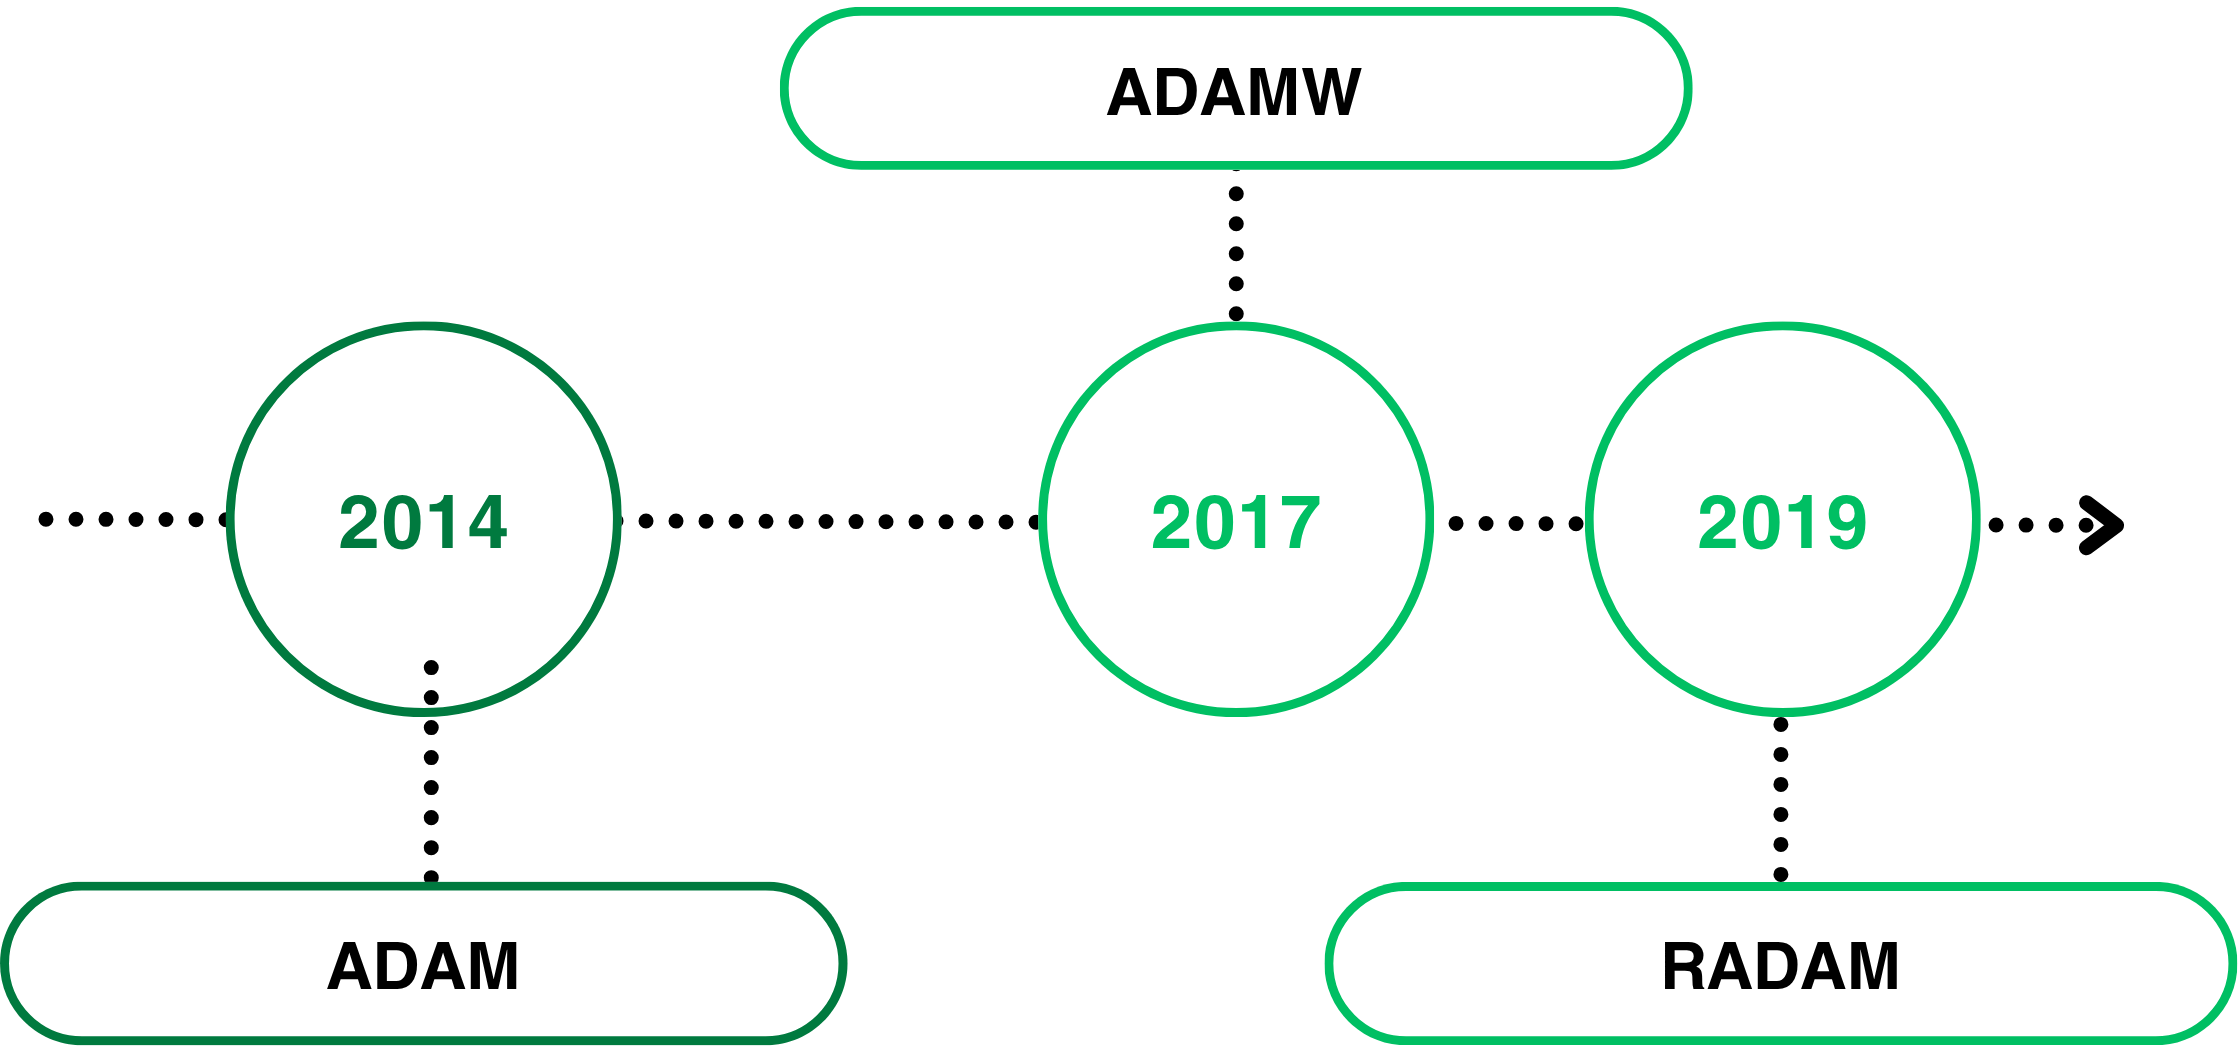
\includegraphics[width=0.7\textwidth]{frise3.png}
  \end{center}

\end{frame}

\begin{frame}{Références}
  \renewcommand*{\bibfont}{\small}
  \printbibliography[heading=none]
\end{frame}

\end{document}